%% LyX 2.3.2 created this file.  For more info, see http://www.lyx.org/.
%% Do not edit unless you really know what you are doing.
\documentclass[12pt]{article}
\usepackage[latin9]{inputenc}
\usepackage[letterpaper]{geometry}
\geometry{verbose,tmargin=1in,bmargin=1in,lmargin=1in,rmargin=1in}
\usepackage{fancyhdr}
\pagestyle{fancy}
\usepackage{float}
\usepackage{mathtools}
\usepackage{bm}
\usepackage{amsmath}
\usepackage{amssymb}
\usepackage{graphicx}
\usepackage{setspace}
\setstretch{1.5}

\makeatletter
%%%%%%%%%%%%%%%%%%%%%%%%%%%%%% User specified LaTeX commands.


% packages
                   	
\usepackage{bm}
%\usepackage[nodisplayskipstretch]{setspace}
\usepackage{enumitem}
\usepackage{fancyheadings}
\usepackage{csquotes}


% Configuration


\input{"../../_HeadersEtc/SESYNCBayes/middle_header.txt"}
\chead{Model Building}
\title{\vspace{-1cm}Model  Building Exercises}

% Custom commands
\newif\ifanswers
%\answerstrue % comment out to hide answers

\makeatother

\begin{document}
\maketitle

\thispagestyle{fancy}

\section{Motivation}

The ability of Bayesian methods to handle hierarchical models in an
unusually tidy way is why they are becoming the first choice for complex
problems in social and environmental science, problems with many unknowns,
different type of data, and multiple sources of uncertainty. Recall
that the posterior distribution of all of the unobserved quantities
is proportionate to the joint distributions of the unobserved quantities
and the data:

\[
\big[\bm{\theta}\mid\mathbf{y}\big]\propto\underbrace{\big[\bm{\theta},\mathbf{y}\big]}_{\mathclap{\text{Factor into sensible parts}}}
\]
It follows that the starting point for developing hierarchical models
is to write a properly factored expression for the proportionality
between the posterior and joint distribution of the observed and unobserved
quantities. Properly means that the expression for the factored joint
distribution obeys the chain rule of probability after assumptions
about independence have been made. Bayesian networks, also called
directed acyclic graphs (or, unattractively in my view, DAGs), offer
a way to visually assure that your model does so. This will be true
if there is one unknown and one data set or one hundred unknowns and
ten data sets. This factored expression is all that is required to
specify a \enquote{roll-your-own} MCMC algorithm or to write code
in one of the current software packages that sample from the marginal
posterior distributions, JAGS, STAN, OpenBUGS etc. The expression
for posterior and joint is where you start discussions with statistical
colleagues. It must be included in all papers and proposals using
Bayesian methods because it communicates virtually everything about
where your inferences come from.

Learning to write proper mathematical and statistical expressions
for Bayesian models is 70 percent of the battle of learning how to
do Bayesian analysis. We will return to this battle time and time
again during this course. In this exercise, we begin to learn the
vital skill of model building. The problems increase in difficulty
as we proceed, so it will be important to understand what you did
right and wrong before you proceed to the next problem. In addition
to practice drawing Bayesian networks and writing posterior and joint
distributions, the problems will challenge you to:
\begin{itemize}
\item Choose distributions appropriate for the support of the random variable. 
\item Deftly use moment matching to convert means and standard deviations
to parameters of distributions.
\end{itemize}

\section{Instructions}
\begin{itemize}
\item For each problem below, draw the Bayesian network, write the posterior
and joint distributions using generic bracket notation with appropriate
products. Next, choose specific distributions following the general
flow that we illustrated in the Light Limitation of Trees lecture.
At this point, don't worry too much about the specific forms for prior
distributions. We will learn more about composing these as the course
proceeds. You may use uniform distributions with bounds that are vague
for non-negative parameters. Use normal distributions centered on
zero with large variances for real-valued parameters. Again, don't
sweat this too much. 
\item Work in groups to allow discussion and to teach each other. Prepare
a write up, one per group. You may use pencil and paper for drawing
DAGs and writing models. Please practice proper notation. Indicate
vectors and matrices by underling their symbols.
\item We urge you to do a problem as completely as you possibly can, then
consult the answer before going to the next problem. 
\item Good for you if you think you found a mistake! There will be some
lurking errors because some of these problems have not been vetted.
There is no better way to show that you are learning than to find
mistakes. 
\item Accumulate questions.
\end{itemize}

\section{Problems}

\subsection{Cover of invasives on transects}

This problem is taken with minor modification from work Tom is doing
for the National Park Service Inventory and Monitoring Program. The
data consist of point intercepts taken at .1 m intervals along 30
meter transects. Each transect has 300 points where observers classify
a point defined by a plumb line dropped vertically from the transect
as intersecting with exotic vegetation, native vegetation, or bare
ground. There are 100 transects. You seek to estimate the proportion
of total vegetative cover that is native using the proportion of a
transect that is bare ground as a predictor variable. Develop a Bayesian
model for this problem that properly models uncertainty in the predictor
variable (proportion bare ground) and the response variable (proportion
exotic cover). Hints - Think about two data models, one for the response
and one for the predictor variable. Model the $x's$ using the same
approach you use for modeling the $y's$ and link the data models
via a latent, unobserved quantity. The sample unit is a transect.
Start by thinking about what is observed, what is unobserved, and
what is known for each transect. 

Define:
\begin{itemize}
\item $y_{i}=$ observed number of hits of exotics on transect $i$
\item $v_{i}=$ number of hits of exotic and native vegetation on transect
\emph{$i$, }presumed to be known because it observed without error.
\item $x_{i}=$ the true, unobserved proportion of bare ground on transect
\emph{i}
\item $w_{i}=$ observed number of hits with bare soil
\item $n_{i}=$ total number of intercepts on a transect, known.
\item $N$ = total number of transects
\end{itemize}


\subsection{Controls on willow seedling establishment}
\begin{enumerate}
\item You are interested in the way that soil water and herbaceous plant
cover influence establishment of willow seedlings in riparian communities.
You have data on the number of willow seedlings that establish on
100 10 $\times$ 10 meter plots, which of course are a random variables
before they are observed. Assume these data are measured perfectly
(i.e., you did not over or under count seedlings). You also have five
measurements of soil water and one measurement of percent herbaceous
cover (estimated visually) on each plot. Assume for now that herbaceous
cover is measured perfectly, but you want to include sampling variation
in soil water for each plot in your model. How would you model the
effect of soil water and herbaceous cover on the number of plants
established?\newpage \newpage
\item A colleague objected to your assumption of cover observed perfectly
by eye, insisting, reasonably we think, that you develop a data model
relating your ocular estimate to the true cover in a plot. So, you
obtained visual estimates of cover paired with the actual proportion
of vegetated area (measured using small sub-plots) on 15 10 x 10 m
plots. After days of sweaty labor, you regressed visual estimates
$(x_{i})$ on the true cover $(z_{i})$ and developed a calibration
equation $h(\bm{\alpha},z_{i})$:
\begin{eqnarray}
h(\bm{\alpha},z_{i}) & = & \frac{e^{\alpha_{o}+\alpha_{1}z_{i}}}{1+e^{\alpha_{o}+\alpha_{1}z_{i}}}\\
x_{i} & \sim & \text{beta}\big(m(h(\bm{\alpha},z_{i}),\varsigma^{2})\big)\\
\alpha_{o} & \sim & \text{\text{normal}(.05,.006)}\\
\alpha_{1} & \sim & \text{normal}(1.07,.13)\\
\varsigma^{2} & \sim & \text{inverse gamma}(10.2,630)
\end{eqnarray}
\item The function $m(\,)$ returns parameters of the beta distribution
given moments as inputs. Include the calibration equation in your
model of effects of soil water and herbaceous cover on seedling establishment
using informed priors on $\alpha_{0},\alpha_{1}$ and $\varsigma^{2}$.
Hint\textendash think about the predictor variable for herbaceous
cover. Do you want to use the observed value of cover $(x_{i})$ or
the true value $(z_{i})$ to model its effect on establishment?
\item 
\item Now presume that the 100 plots are arranged in 5 different stream
reaches, 20 plots in each reach. You have data on peak runoff in each
of the reaches, which you may assume is measured perfectly. Describe
verbally how you might model variation at the catchment scale created
by peak runoff. 
\end{enumerate}

\subsection{Effect of radon on cancer risk}

You seek to understand how radon levels influence risk of cancer.
You have data on the incidence of lung cancer in households (1 if
cancer is present and 0 if no cancer) and radon levels (a continuous,
non-negative number) for 1000 houses in each of 40 counties within
a state. You also have data on the clay soil content at the county
level. You heroically assume both clay content and radon levels are
know without error. How would you model the effect of radon and soil
type on the probability of lung cancer? Some hints\textendash{}
\begin{enumerate}
\item What deterministic model would you use to predict the probability
of cancer in a household as a function of radon level? 
\item What likelihood would you use for these 0 or 1 data? 
\item Assume that the intercept in your deterministic model of the effect
of radon level on probability of cancer in a household is a linear
function of county level clay soil content.

\ifanswers 
\begin{figure}[H]
\center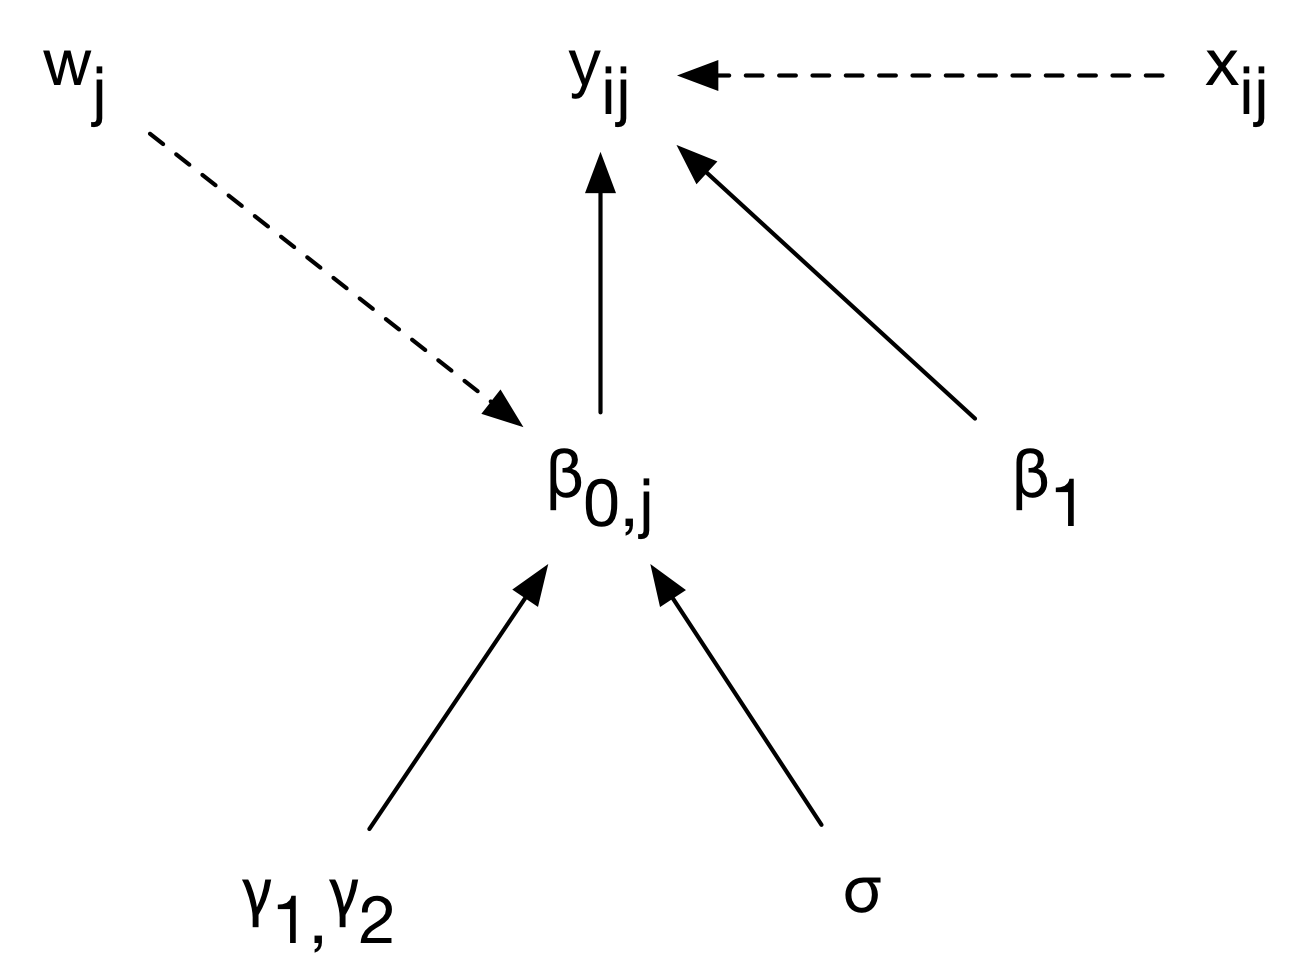
\includegraphics[width=2.75in]{../../../../../SESYNCBayes/Labs/ModelBuilding/RadonDAG}
\caption{In this DAG, $x_{ij}$ is the radon level and $y_{ij}$ is an indicator
that equals 1 if cancer is present and 0 if it is not in the $i_{\textrm{th}}$
house in the $j_{\textrm{th}}$ county, and $w_{\textrm{th}}$ is
the clay soil content in the $j_{\textrm{th}}$ county.}
\end{figure}

\begin{align*}
\big[\bm{\gamma},\bm{\beta},\sigma\mid\bm{y}\big]\varpropto\prod_{i=1}^{1000}\prod_{j=1}^{40}\big[y_{ij}\mid g\big(\bm{\beta},x_{ij}\big)\big]\big[\beta_{0,j}\mid h\big(\bm{\gamma},w_{j}\big),\sigma^{2}\big]\big[\bm{\gamma}\big]\big[\beta_{1}\big]\big[\sigma\big]
\end{align*}
\[
\begin{aligned} & g\big(\bm{\beta},x_{ij}\big)=\frac{e^{\beta_{0,j}+\beta_{1}x_{ij}}}{1+e^{\beta_{0,j}+\beta_{1}x_{ij}}}\\
 & h\big(\bm{\gamma},w_{j}\big)=\gamma_{0}+\gamma_{1}w_{j}\\
 & y_{ij}\sim\textrm{Bernoulli}\big(g\big(\bm{\beta},x_{ij}\big)\big)\\
 & \beta_{0,j}\sim\textrm{normal}\big(h\big(\bm{\gamma},w_{j}\big),\sigma^{2})\\
 & \beta_{1}\sim\textrm{normal}\big(0,1000)
\end{aligned}
\quad\quad\quad\begin{aligned} & \gamma_{0}\sim\textrm{normal}\big(0,1000)\\
 & \gamma_{1}\sim\textrm{normal}\big(0,1000)\\
 & \sigma\sim\textrm{uniform}\big(0,1000)\\
\\
\\
\end{aligned}
\]
\newpage\fi
\end{enumerate}

\end{document}
